%%%%%%%%%%%%%%%%%%%%%%%%%%%%%%%
%%%%%%      Section      %%%%%%
%%%%%%%%%%%%%%%%%%%%%%%%%%%%%%%
\section{Concept and definitions}\label{sec:git}
Local repo. consists of following 3 "trees" maintained by git.
\begin{enumerate}\packed
\item \TT{Working Directory} holds the actual files.
\item \TT{Index} = \TT{staging area}.
\item \TT{Head} = last commit.
\end{enumerate}
\setdescription{labelsep=\textwidth}
\begin{center}
	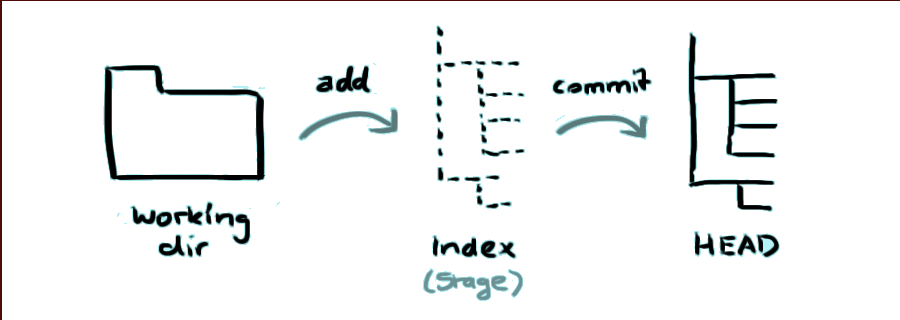
\includegraphics[trim=.5in 0in 0in 0.2in, clip=true,
	keepaspectratio=true, width=.6\textwidth]{./img/trees.png}
	\nl Courtesy of \url{https://rogerdudler.github.io/git-guide/}
\end{center}